% =============================================================================
%  The assumptions of a one-dimensional PBL closure, as a pyramid -- VERTICAL, COLOUR-CODED version
%  GENERATED by scripts/make_pyramid_colour.py from pbl_assumptions_pyramid_split_vertical.tex (itself generated by make_pyramid_vertical.py from pbl_assumptions_pyramid_split.tex; edit the
%  horizontal file and regenerate. Tiers are columns (physics | concepts | formalism); a block
%  touches at its left exactly what it relies on. Scale: 0.86 cm per old cm along the ground,
%  column widths [2.5, 4.18, 5.3] cm for premises, concepts, formalism. Build: tectonic pbl_assumptions_pyramid_vertical.tex
% =============================================================================
\documentclass[10pt]{article}
\usepackage{iftex}
\ifPDFTeX
  \usepackage[utf8]{inputenc}
  \usepackage[T1]{fontenc}
  \usepackage{lmodern}
\else
  \usepackage{fontspec}
  \setmainfont{lmroman10-regular.otf}[BoldFont=lmroman10-bold.otf,
    ItalicFont=lmroman10-italic.otf, BoldItalicFont=lmroman10-bolditalic.otf]
\fi
\usepackage[british]{babel}
\usepackage[a4paper,margin=9mm,top=9mm,bottom=9mm]{geometry}
\usepackage{amsmath,amssymb}
\usepackage{xcolor}
\usepackage{tikz}
\usepackage{microtype}
\pagestyle{empty}
\setlength{\parindent}{0pt}
\setlength{\parskip}{0.5ex}
% rigid math relation spacing: the centred block texts would otherwise stretch around = and <<
\thickmuskip=5mu \medmuskip=4mu \thinmuskip=3mu

% ---- notation ---------------------------------------------------------------
\newcommand{\avg}[1]{\langle #1 \rangle}
\newcommand{\pd}[2]{\partial #1/\partial #2}
\newcommand{\qsq}{q^{2}}
\newcommand{\Rfc}{R_{fc}}
\newcommand{\dx}{\Delta x}
% ---- rows the PhD concept turns on (same data as the note's macros.tex) ------
\definecolor{cKey}{HTML}{7B2D8E}
\definecolor{cGXIX}{HTML}{990011}   % Goger 2019 port (the note's colour)
\definecolor{cFULL}{HTML}{7B2D8E}   % Kosovic-Juliano 3D closure (the note's colour)
% \hl{x0}{x1}{y0}{y1}{colour}{inset}: a frame inside a block, marking a scheme's decisive block
\newcommand{\hl}[6]{\draw[#5, line width=1.1pt] (#1+#6,#3+#6) rectangle (#2-#6,#4-#6);}
\newcommand{\setkey}[2]{\expandafter\def\csname key@#1\endcsname{#2}}
\makeatletter
\setkey{A1}{1}\setkey{B1}{1}\setkey{B2}{1}\setkey{B3}{1}\setkey{C3}{1}\setkey{C4}{1}\setkey{C6}{1}\setkey{C7}{1}
\setkey{B5}{2}\setkey{B6}{2}\setkey{C2}{2}\setkey{C5}{2}\setkey{C9}{2}
\newcommand{\keymark}[1]{\ifcsname key@#1\endcsname
  \if1\csname key@#1\endcsname\textcolor{cKey}{$\blacktriangleright$}\else\textcolor{cKey}{$\triangleright$}\fi\fi}
\makeatother
\newcommand{\pid}[1]{\keymark{#1}\textbf{#1}}
% \pb{x0}{x1}{y0}{y1}{style}{text}: a block from (x0,y0) to (x1,y1), text centred
\newcommand{\pbf}[7]{\pgfmathsetmacro{\pbw}{#2-#1-#7}%
  \draw[#5] (#1,#3) rectangle (#2,#4);
  \node[align=center, font=\tiny, inner sep=0pt, text width=\pbw cm] at ({(#1+#2)/2},{(#3+#4)/2}) {#6};}
% \pbunion{style}{tx}{ty}{tw}{text}{pieces x0/x1/y0/y1,...}{outline (x,y) -- ...}: one block of several rectangles
\newcommand{\pbunion}[7]{\foreach \ux/\uX/\uy/\uY in {#6} {\fill[black!22] (\ux,\uy) rectangle (\uX,\uY);}
  \draw[#1, fill=none] #7 -- cycle;
  \node[align=center, font=\tiny, inner sep=0pt, text width=#4 cm] at (#2,#3) {#5};}
\newcommand{\pb}[6]{\pgfmathsetmacro{\pbw}{#2-#1-0.20}%
  \draw[#5] (#1,#3) rectangle (#2,#4);
  \node[align=center, font=\tiny, inner sep=0pt, text width=\pbw cm] at ({(#1+#2)/2},{(#3+#4)/2}) {#6};}


% ---- the hectometre-scale column (used by the VERTICAL version only; read by scripts/make_pyramid_vertical.py)
% \hecto{<formal statement title>}{<what becomes of it at Delta = 500 m over the Inn Valley>}; no-op here.
% Sources: the mountain and grey-zone columns of the note's Table I.1 and the project's own runs.
\newcommand{\hecto}[2]{}
\hecto{Grid means are ensemble means}{By day much of the kinetic energy at the lowest levels is resolved, the effective resolution is several $\Delta$, and the partition claim waits for a $w$-spectrum below that scale; the resolved shear then enters production twice. At night the eddies shrink far below $\Delta$: the cell holds only a few integral scales and the vertical grid none, the cell statistic is a single realisation, and the stable regime is mesoscale again. On a slope the cell mixes slope layer and valley core.}
\hecto{Vertical shear only}{The jet's cross-valley shear is a sizeable fraction of its vertical shear; in weak drainage flow directional shear sets $u_*$.}
\hecto{Vertical divergence only}{Horizontal flux divergences are of the order of the vertical one, and the Riviera budgets closed only with transport and advection; the numerical operator stands where the physical divergence belongs, and the energy it removes vanishes instead of feeding $\qsq$.}
\hecto{Wall value of $\qsq$}{The nocturnal sonics record turbulence at the surface where every model goes laminar; the observed friction velocity implies a wall $\qsq$ between the two closures' values.}
\hecto{Level-2.5 truncation}{The closure's own ordering justifies the step in stable and slightly unstable air, not toward free convection. Transitions outrun $l/q$; the strain cap's footprint measures it.}
\hecto{Stability functions and cutoff}{Most nocturnal valley cells lie beyond the critical Richardson number, where the deficit against the control is flat; the approximate closure switches off at $\Rfc$, the others never.}
\hecto{Surface fluxes and first level}{The katabatic jet maximum sits inside the layer; over forest the first level lies in the roughness sublayer; the momentum flux is rarely height-constant.}
\hecto{Master length scale}{$z_i$ is ill-posed under elevated inversions, the wall distance ambiguous on a slope, the horizontal eddy set by the valley width: two lengths. In the cold pool the length, not the fluxes, was the lever; the fork bounds it by a buoyancy limit and a strain cap.}
\hecto{Constant set}{Three constant sets in one comparison; their dissipation constants differ by a factor that rivals the effects to be reported.}
\hecto{One length for $K$ and $\varepsilon$}{$\varepsilon$ is filter-independent while $q^3$ is not, so the dissipation length must shrink with the grid; the inertial-subrange estimate from the sonics needs Taylor's hypothesis and fails in weak-wind nights.}
\hecto{Pressure terms}{Taking them small is ``a dangerous assumption'' in complex terrain; the Radfeld budget residual is their only observation.}
\hecto{K-form fluxes}{By day the eddies span $z_i$ and heat runs against the local gradient: the plume terms exist for this. Where slope wind turns into valley wind the stress axes leave the gradient and the jet veers with height: $\avg{uv}$ appears, negative production is admissible. The grid filter, aspect ratio 25, imprints its anisotropy on the subgrid eddies; in stable air $K_H/K_M$ falls with Ri.}
\hecto{Buoyancy term}{The slope-normal surface heat flux has a horizontal component with no home in the budget; in stable air buoyancy damps $\avg{w^2}$ selectively; on fog nights the saturated flux follows the moist gradient, which only the control's condensation scheme knows; $\beta = 1/300$~K is a few percent off at valley $\Theta_v$.}

% ---- dependencies the contact rule cannot draw (post-audit list; used by scripts/make_pyramid_graph.py). No-op here.
\newcommand{\lean}[2]{}
\lean{Boundary-layer (column) approximation}{Boussinesq}
\lean{Energy cascade}{Stationarity}
\lean{Local equilibrium}{Locality}
\lean{Local equilibrium}{Horizontal homogeneity}
\lean{Monin--Obukhov similarity}{Constant-flux layer}
\lean{Mixing length}{Mixing}
\lean{Locality}{Mixing}
\lean{Energy cascade}{Mixing}
\lean{Eddy viscosity}{Locality}
\lean{Eddy viscosity}{Mixing length}
\lean{Return to isotropy}{Horizontal homogeneity}
\lean{Stability functions and cutoff}{Level-2.5 truncation}
\lean{Level-2.5 truncation}{Weak anisotropy}
\lean{Buoyancy production}{Return to isotropy}
\lean{Universal constants}{Reynolds decomposition}
\lean{Vertical divergence only}{Spectral gap}
\lean{Wall value of $\qsq$}{Universal constants}
\lean{Stability functions and cutoff}{Universal constants}
\lean{Stability functions and cutoff}{Boundary-layer (column) approximation}
\lean{Stability functions and cutoff}{Buoyancy production}
\lean{Stability functions and cutoff}{Local equilibrium}
\lean{Master length scale}{Buoyancy term}
\lean{Buoyancy term}{K-form fluxes}
\lean{Pressure terms}{Locality}
\lean{Pressure terms}{Universal constants}
\lean{One length for $K$ and $\varepsilon$}{Master length scale}
\lean{K-form fluxes}{Master length scale}
\lean{K-form fluxes}{Stability functions and cutoff}
% ---- scheme quicklook (moons above the formalism tier; scripts/make_moons.py rewrites the strip)
% \moon{<block title>}{K|P|D x4} in the order MYNN as run, G19 port, 3D-APPROX, 3D-FULL; from Table I.0 of the note:
% a block is K if all its rows are kept, D if all are dropped, else P. No-op here (data only).
\newcommand{\moon}[2]{}
\moon{Grid means are ensemble means}{P K P P}
\moon{Vertical shear only}{K P K D}
\moon{Vertical divergence only}{K P P D}
\moon{Wall value of $\qsq$}{K K D D}
\moon{Level-2.5 truncation}{K K K K}
\moon{Stability functions and cutoff}{D P K P}
\moon{Surface fluxes and first level}{K K K K}
\moon{Master length scale}{K P K K}
\moon{Constant set}{K K K K}
\moon{One length for $K$ and $\varepsilon$}{K K K K}
\moon{Pressure terms}{K K K K}
\moon{K-form fluxes}{P P P D}
\moon{Buoyancy term}{P P P P}
% glyphs (the note's), absolute size, colour = scheme identity
\newcommand{\gK}{\tikz[baseline=-0.6ex]{\fill (0,0) circle (0.11);}}
\newcommand{\gP}{\tikz[baseline=-0.6ex]{\draw[line width=0.5pt] (0,0) circle (0.11); \fill (0,0) -- (90:0.11) arc (90:270:0.11) -- cycle;}}
\newcommand{\gD}{\tikz[baseline=-0.6ex]{\draw[line width=0.5pt] (0,0) circle (0.11);}}
\definecolor{cMYNN}{HTML}{3A6B00}    % MYNN as run
\definecolor{cAPPROX}{HTML}{9A5AA8}  % 3D-APPROX


% vertical block: rectangle + centred text, text width = block width - hpad
\newcommand{\pbv}[7]{\pgfmathsetmacro{\pbw}{#2-#1-#7}%
  \draw[#5] (#1,#3) rectangle (#2,#4);
  \node[align=center, font=\fontsize{7}{7.5}\selectfont, inner sep=0pt, text width=\pbw cm] at ({(#1+#2)/2},{(#3+#4)/2}) {#6};}
\newcommand{\hlv}[6]{\draw[#5, line width=1.1pt] (#1+#6,#3+#6) rectangle (#2-#6,#4-#6);}
% compound blocks in the page's text size
\renewcommand{\pbunion}[7]{\foreach \ux/\uX/\uy/\uY in {#6} {\fill[#1] (\ux,\uy) rectangle (\uX,\uY);}
  \draw[bk] #7 -- cycle;
  \node[align=center, font=\fontsize{7}{7.5}\selectfont, inner sep=0pt, text width=#4 cm] at (#2,#3) {#5};}
% hectometre box: dashed, left-aligned commentary beside a concept (not a block of the chain)
\newcommand{\pbh}[5]{\pgfmathsetmacro{\pbw}{#2-#1-0.30}%
  \draw[hecto] (#1,#3) rectangle (#2,#4);
  \node[align=left, font=\fontsize{6.5}{7.6}\selectfont, inner sep=0pt, text width=\pbw cm] at ({(#1+#2)/2},{(#3+#4)/2}) {#5};}

% ---- block colours (OKLCH: hue by vertical position, lightness by column) ----
\definecolor{blk0}{rgb}{0.9978,0.8786,0.8520} % Spectral gap
\definecolor{blk1}{rgb}{0.9901,0.8850,0.8309} % Mixing
\definecolor{blk2}{rgb}{0.7796,0.9775,0.6880} % Stationarity
\definecolor{blk3}{rgb}{0.5816,0.9961,0.9530} % Similarity
\definecolor{blk4}{rgb}{0.9945,0.8999,0.6849} % Horizontal homogeneity
\definecolor{blk5}{rgb}{0.7851,0.9388,0.9949} % Small-scale isotropy
\definecolor{blk6}{rgb}{0.8539,0.9169,0.9878} % Weak anisotropy
\definecolor{blk7}{rgb}{0.8771,0.9080,0.9911} % Gradient scale
\definecolor{blk8}{rgb}{0.9057,0.8959,0.9975} % Axisymmetric mixing
\definecolor{blk9}{rgb}{0.9476,0.8784,0.9986} % Boussinesq
\definecolor{blk10}{rgb}{0.9958,0.6757,0.6067} % Reynolds decomposition
\definecolor{blk11}{rgb}{0.9853,0.6948,0.4904} % Ergodicity in space
\definecolor{blk12}{rgb}{0.8762,0.7579,0.4257} % Boundary-layer (column) approximation
\definecolor{blk13}{rgb}{0.7500,0.8060,0.4741} % Constant-flux layer
\definecolor{blk14}{rgb}{0.6512,0.8322,0.5444} % Local equilibrium
\definecolor{blk15}{rgb}{0.5014,0.8562,0.6747} % Monin--Obukhov similarity
\definecolor{blk16}{rgb}{0.4003,0.8607,0.7884} % Mixing length
\definecolor{blk17}{rgb}{0.3656,0.8526,0.8837} % Universal constants
\definecolor{blk18}{rgb}{0.4078,0.8330,0.9660} % Energy cascade
\definecolor{blk19}{rgb}{0.5563,0.7977,0.9942} % Return to isotropy
\definecolor{blk20}{rgb}{0.7291,0.7435,0.9947} % Eddy viscosity
\definecolor{blk21}{rgb}{0.6693,0.7660,0.9890} % Locality
\definecolor{blk22}{rgb}{0.8310,0.6990,0.9964} % Buoyancy production
\definecolor{blk23}{rgb}{0.8370,0.5378,0.3703} % Grid means are ensemble means
\definecolor{blk24}{rgb}{0.7680,0.5859,0.2824} % Vertical shear only
\definecolor{blk25}{rgb}{0.6945,0.6223,0.2792} % Vertical divergence only
\definecolor{blk26}{rgb}{0.5892,0.6600,0.3372} % Wall value of $\qsq$
\definecolor{blk27}{rgb}{0.4894,0.6843,0.4140} % Level-2.5 truncation
\definecolor{blk28}{rgb}{0.3599,0.7028,0.5203} % Surface fluxes and first level
\definecolor{blk29}{rgb}{0.2289,0.7081,0.6333} % Master length scale
\definecolor{blk30}{rgb}{0.1693,0.7001,0.7300} % Constant set
\definecolor{blk31}{rgb}{0.2112,0.6865,0.7922} % One length for $K$ and $\varepsilon$
\definecolor{blk32}{rgb}{0.3157,0.6625,0.8509} % Pressure terms
\definecolor{blk33}{rgb}{0.4082,0.6386,0.8804} % Stability functions and cutoff
\definecolor{blk34}{rgb}{0.5461,0.5972,0.8886} % K-form fluxes
\definecolor{blk35}{rgb}{0.6821,0.5514,0.8377} % Buoyancy term
\begin{document}
{\large\bfseries The assumptions of a one-dimensional PBL closure, as a pyramid: what rests on what}\\[0.2ex]
{\small Colour-coded page of the split variant, 2026-09-21: spectral gap and gradient scale as separate premises. 2026-09-17.}

\vspace{0.3ex}
{\footnotesize Left the premises, middle the concepts of turbulence theory, right the formal statements of the level-2.5 closure; a block touches at its left exactly the blocks it relies on. \textbf{Colour names a place}: the hue by height on the page, red at the top to violet at the bottom, the shade darkening from left to right. \textbf{A corner triangle} marks a dependence no contact can show, in the colour of the block depended on: left corners point to the previous column, right corners to the same column, upper to a block above, lower to one below. Dashed: each formal statement at $\Delta = 500$~m over the Inn Valley; far right the schemes \textcolor{cMYNN}{\textbf{MYNN as run}}, \textcolor{cGXIX}{\textbf{G19 port}}, \textcolor{cAPPROX}{\textbf{3D-APPROX}}, \textcolor{cFULL}{\textbf{3D-FULL}}, \gK{} implements, \gP{} partly, \gD{} drops. Rules, reading and the list of triangles overleaf.\par}

\vspace{0.4ex}
\begin{center}
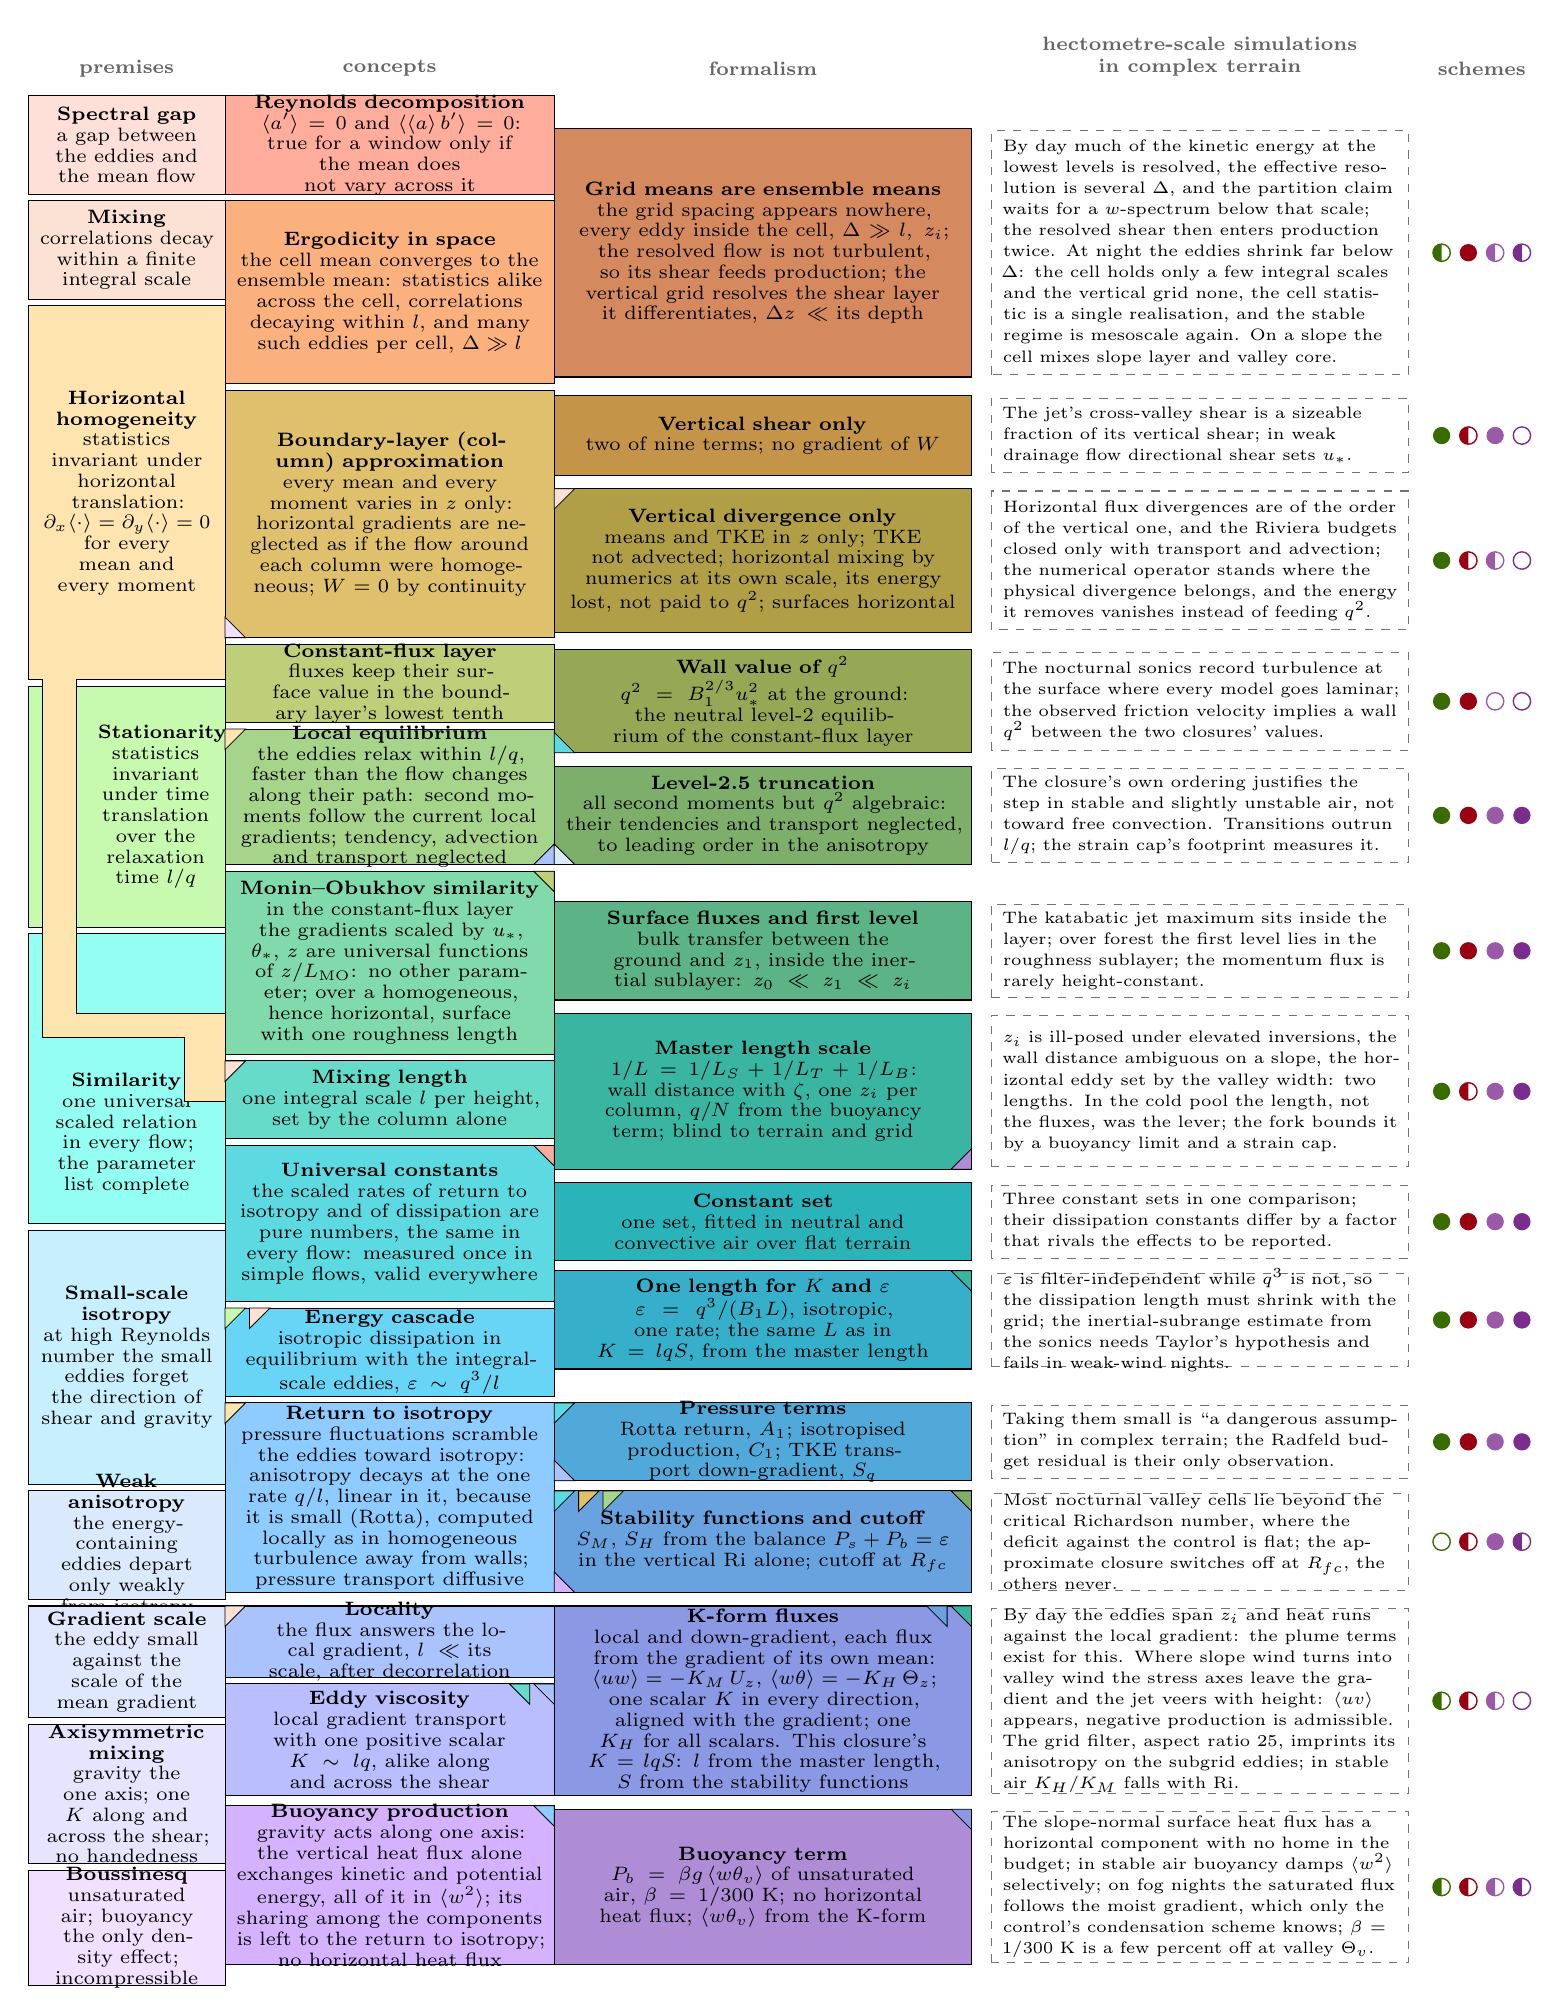
\begin{tikzpicture}[x=1cm, y=1cm,
  ground/.style={draw, line width=0.4pt, fill=black!22},
  hyp/.style={draw, line width=0.4pt, fill=black!9},
  row/.style={draw, line width=0.4pt, fill=white},
  bk/.style={draw, line width=0.4pt},
  hecto/.style={draw=black!55, dashed, line width=0.4pt, fill=white}]
\node[font=\scriptsize\bfseries, text=black!60] at (1.250,23.871) {premises};
\node[font=\scriptsize\bfseries, text=black!60] at (4.590,23.871) {concepts};
\node[font=\scriptsize\bfseries, text=black!60] at (9.330,23.871) {formalism};
\node[font=\scriptsize\bfseries, text=black!60] at (18.460,23.871) {schemes};
\node[font=\scriptsize\bfseries, text=black!60, align=center] at (14.880,24.021) {hectometre-scale simulations\\ in complex terrain};
\pbv{0.000}{2.500}{22.274}{23.521}{bk, fill=blk0}{\textbf{Spectral gap}\\ a gap between the eddies and the mean flow}{0.30}
\pbv{0.000}{2.500}{20.941}{22.188}{bk, fill=blk1}{\textbf{Mixing}\\ correlations decay within a finite integral scale}{0.30}
\pbunion{blk2}{1.618}{14.491}{1.46}{\textbf{Stationarity}\\ statistics invariant under time translation over the relaxation time $l/q$}{0.735/2.500/12.965/16.018,0.000/0.735/12.965/16.018}{(0.000,16.018) -- (2.500,16.018) -- (2.500,12.965) -- (0.000,12.965)}
\pbunion{blk3}{1.250}{10.342}{2.20}{\textbf{Similarity}\\ one universal scaled relation in every flow; the parameter list complete}{0.000/2.500/9.202/11.481,0.000/2.500/11.481/12.879}{(0.000,12.879) -- (2.500,12.879) -- (2.500,9.202) -- (0.000,9.202)}
\pbunion{blk4}{1.250}{18.479}{2.20}{\textbf{Horizontal homogeneity}\\ statistics invariant under horizontal translation: \mbox{$\partial_x\avg{\cdot} = \partial_y\avg{\cdot} = 0$} for every mean and every moment}{0.000/2.500/16.104/20.855,0.176/0.618/11.567/16.104,0.176/2.500/11.567/11.868,1.985/2.500/10.750/11.868}{(0.000,20.855) -- (2.500,20.855) -- (2.500,16.104) -- (0.618,16.104) -- (0.618,11.868) -- (2.500,11.868) -- (2.500,10.750) -- (1.985,10.750) -- (1.985,11.567) -- (0.176,11.567) -- (0.176,16.104) -- (0.000,16.104)}
\pbv{0.000}{2.500}{5.891}{9.116}{bk, fill=blk5}{\textbf{Small-scale isotropy}\\ at high Reynolds number the small eddies forget the direction of shear and gravity}{0.30}
\pbv{0.000}{2.500}{4.429}{5.805}{bk, fill=blk6}{\textbf{Weak anisotropy}\\ the energy-containing eddies depart only weakly from isotropy}{0.30}
\pbv{0.000}{2.500}{2.924}{4.343}{bk, fill=blk7}{\textbf{Gradient scale}\\ the eddy small against the scale of the mean gradient}{0.30}
\pbv{0.000}{2.500}{1.075}{2.838}{bk, fill=blk8}{\textbf{Axisymmetric mixing}\\ gravity the one axis; one $K$ along and across the shear; no handedness}{0.30}
\pbv{0.000}{2.500}{-0.473}{0.989}{bk, fill=blk9}{\textbf{Boussinesq}\\ unsaturated air; buoyancy the only density effect; incompressible}{0.30}
\pbv{2.500}{6.680}{22.274}{23.521}{bk, fill=blk10}{\textbf{Reynolds decomposition}\\ $\avg{a'} = 0$ and $\avg{\avg{a}\,b'} = 0$:\\ true for a window only if\\ the mean does not vary across it}{0.30}
\pbv{2.500}{6.680}{19.866}{22.188}{bk, fill=blk11}{\textbf{Ergodicity in space}\\ the cell mean converges to the ensemble mean: statistics alike across the cell, correlations decaying within $l$, and many such eddies per cell, \mbox{$\Delta \gg l$}}{0.30}
\pbv{2.500}{6.680}{16.641}{19.780}{bk, fill=blk12}{\textbf{Boundary-layer (column) approximation}\\ every mean and every moment varies in $z$ only: horizontal gradients are neglected as if the flow around each column were homogeneous; $W = 0$ by continuity}{0.56}
\pbv{2.500}{6.680}{15.566}{16.555}{bk, fill=blk13}{\textbf{Constant-flux layer}\\ fluxes keep their surface value in the boundary layer's lowest tenth}{0.30}
\pbv{2.500}{6.680}{13.760}{15.480}{bk, fill=blk14}{\textbf{Local equilibrium}\\ the eddies relax within $l/q$, faster than the flow changes along their path: second moments follow the current local gradients; tendency, advection and transport neglected}{0.30}
\pbv{2.500}{6.680}{11.352}{13.674}{bk, fill=blk15}{\textbf{Monin--Obukhov similarity}\\ in the constant-flux layer the gradients scaled by $u_*$, $\theta_*$, $z$ are universal functions of $z/L_{\mathrm{MO}}$: no other parameter; over a homogeneous, hence horizontal, surface with one roughness length}{0.30}
\pbv{2.500}{6.680}{10.277}{11.266}{bk, fill=blk16}{\textbf{Mixing length}\\ one integral scale $l$ per height, set by the column alone}{0.30}
\pbv{2.500}{6.680}{8.213}{10.191}{bk, fill=blk17}{\textbf{Universal constants}\\ the scaled rates of return to isotropy and of dissipation are pure numbers, the same in every flow: measured once in simple flows, valid everywhere}{0.30}
\pbv{2.500}{6.680}{7.009}{8.127}{bk, fill=blk18}{\textbf{Energy cascade}\\ isotropic dissipation in equilibrium with the integral-scale eddies, $\varepsilon \sim q^3/l$}{0.30}
\pbv{2.500}{6.680}{4.515}{6.923}{bk, fill=blk19}{\textbf{Return to isotropy}\\ pressure fluctuations scramble the eddies toward isotropy: anisotropy decays at the one rate $q/l$, linear in it, because it is small (Rotta), computed locally as in homogeneous turbulence away from walls; pressure transport diffusive}{0.30}
\pbv{2.500}{6.680}{1.935}{3.354}{bk, fill=blk20}{\textbf{Eddy viscosity}\\ local gradient transport with one positive scalar $K \sim l q$, alike along and across the shear}{0.40}
\pbv{2.500}{6.680}{3.440}{4.343}{bk, fill=blk21}{\textbf{Locality}\\ the flux answers the local gradient, $l \ll$ its scale, after decorrelation}{0.30}
\pbv{2.500}{6.680}{-0.215}{1.806}{bk, fill=blk22}{\textbf{Buoyancy production}\\ gravity acts along one axis: the vertical heat flux alone exchanges kinetic and potential energy, all of it in $\avg{w^2}$; its sharing among the components is left to the return to isotropy; no horizontal heat flux}{0.30}
\pbv{6.680}{11.980}{19.952}{23.108}{bk, fill=blk23}{\textbf{Grid means are ensemble means}\\ the grid spacing appears nowhere, every eddy inside the cell, $\Delta \gg l,\ z_i$; the resolved flow is not turbulent, so its shear feeds production; the vertical grid resolves the shear layer it differentiates, $\Delta z \ll$ its depth}{0.30}
\pbv{6.680}{11.980}{18.705}{19.711}{bk, fill=blk24}{\textbf{Vertical shear only}\\ two of nine terms; no gradient of $W$}{0.56}
\pbv{6.680}{11.980}{16.710}{18.533}{bk, fill=blk25}{\textbf{Vertical divergence only}\\ means and TKE in $z$ only; TKE not advected; horizontal mixing by numerics at its own scale, its energy lost, not paid to $\qsq$; surfaces horizontal}{0.40}
\pbv{6.680}{11.980}{15.179}{16.486}{bk, fill=blk26}{\textbf{Wall value of $\qsq$}\\ $\qsq = B_1^{2/3} u_*^2$ at the ground: the neutral level-2 equilibrium of the constant-flux layer}{0.30}
\pbv{6.680}{11.980}{13.760}{15.007}{bk, fill=blk27}{\textbf{Level-2.5 truncation}\\ all second moments but $\qsq$ algebraic: their tendencies and transport neglected, to leading order in the anisotropy}{0.30}
\pbv{6.680}{11.980}{12.040}{13.287}{bk, fill=blk28}{\textbf{Surface fluxes and first level}\\ bulk transfer between the ground and $z_1$, inside the inertial sublayer: $z_0 \ll z_1 \ll z_i$}{0.30}
\pbv{6.680}{11.980}{9.890}{11.868}{bk, fill=blk29}{\textbf{Master length scale}\\ $1/L = 1/L_S + 1/L_T + 1/L_B$: wall distance with $\zeta$, one $z_i$ per column, $q/N$ from the buoyancy term; blind to terrain and grid}{0.56}
\pbv{6.680}{11.980}{8.729}{9.718}{bk, fill=blk30}{\textbf{Constant set}\\ one set, fitted in neutral and convective air over flat terrain}{0.30}
\pbv{6.680}{11.980}{7.353}{8.600}{bk, fill=blk31}{\textbf{One length for $K$ and $\varepsilon$}\\ $\varepsilon = q^3/(B_1 L)$, isotropic, one rate; the same $L$ as in $K = lqS$, from the master length}{0.30}
\pbv{6.680}{11.980}{5.934}{6.923}{bk, fill=blk32}{\textbf{Pressure terms}\\ Rotta return, $A_1$; isotropised production, $C_1$; TKE transport down-gradient, $S_q$}{0.30}
\pbv{6.680}{11.980}{4.515}{5.805}{bk, fill=blk33}{\textbf{Stability functions and cutoff}\\ $S_M$, $S_H$ from the balance $P_s + P_b = \varepsilon$\\ in the vertical Ri alone; cutoff at $\Rfc$}{0.56}
\pbv{6.680}{11.980}{1.935}{4.343}{bk, fill=blk34}{\textbf{K-form fluxes}\\ local and down-gradient, each flux from the gradient of its own mean: \mbox{$\avg{uw} = -K_M\,U_z$}, \mbox{$\avg{w\theta} = -K_H\,\Theta_z$}; one scalar $K$ in every direction, aligned with the gradient; one $K_H$ for all scalars. This closure's $K = lqS$: $l$ from the master length, $S$ from the stability functions}{0.40}
\pbv{6.680}{11.980}{-0.215}{1.763}{bk, fill=blk35}{\textbf{Buoyancy term}\\ $P_b = \beta g\,\avg{w\theta_v}$ of unsaturated air, $\beta = 1/300$~K; no horizontal heat flux; $\avg{w\theta_v}$ from the K-form}{0.30}
\node[inner sep=0pt] at (17.950,21.530) {\color{cMYNN}\gP};
\node[inner sep=0pt] at (18.290,21.530) {\color{cGXIX}\gK};
\node[inner sep=0pt] at (18.630,21.530) {\color{cAPPROX}\gP};
\node[inner sep=0pt] at (18.970,21.530) {\color{cFULL}\gP};
\node[inner sep=0pt] at (17.950,19.208) {\color{cMYNN}\gK};
\node[inner sep=0pt] at (18.290,19.208) {\color{cGXIX}\gP};
\node[inner sep=0pt] at (18.630,19.208) {\color{cAPPROX}\gK};
\node[inner sep=0pt] at (18.970,19.208) {\color{cFULL}\gD};
\node[inner sep=0pt] at (17.950,17.621) {\color{cMYNN}\gK};
\node[inner sep=0pt] at (18.290,17.621) {\color{cGXIX}\gP};
\node[inner sep=0pt] at (18.630,17.621) {\color{cAPPROX}\gP};
\node[inner sep=0pt] at (18.970,17.621) {\color{cFULL}\gD};
\node[inner sep=0pt] at (17.950,15.833) {\color{cMYNN}\gK};
\node[inner sep=0pt] at (18.290,15.833) {\color{cGXIX}\gK};
\node[inner sep=0pt] at (18.630,15.833) {\color{cAPPROX}\gD};
\node[inner sep=0pt] at (18.970,15.833) {\color{cFULL}\gD};
\node[inner sep=0pt] at (17.950,14.384) {\color{cMYNN}\gK};
\node[inner sep=0pt] at (18.290,14.384) {\color{cGXIX}\gK};
\node[inner sep=0pt] at (18.630,14.384) {\color{cAPPROX}\gK};
\node[inner sep=0pt] at (18.970,14.384) {\color{cFULL}\gK};
\node[inner sep=0pt] at (17.950,12.664) {\color{cMYNN}\gK};
\node[inner sep=0pt] at (18.290,12.664) {\color{cGXIX}\gK};
\node[inner sep=0pt] at (18.630,12.664) {\color{cAPPROX}\gK};
\node[inner sep=0pt] at (18.970,12.664) {\color{cFULL}\gK};
\node[inner sep=0pt] at (17.950,10.879) {\color{cMYNN}\gK};
\node[inner sep=0pt] at (18.290,10.879) {\color{cGXIX}\gP};
\node[inner sep=0pt] at (18.630,10.879) {\color{cAPPROX}\gK};
\node[inner sep=0pt] at (18.970,10.879) {\color{cFULL}\gK};
\node[inner sep=0pt] at (17.950,9.224) {\color{cMYNN}\gK};
\node[inner sep=0pt] at (18.290,9.224) {\color{cGXIX}\gK};
\node[inner sep=0pt] at (18.630,9.224) {\color{cAPPROX}\gK};
\node[inner sep=0pt] at (18.970,9.224) {\color{cFULL}\gK};
\node[inner sep=0pt] at (17.950,7.976) {\color{cMYNN}\gK};
\node[inner sep=0pt] at (18.290,7.976) {\color{cGXIX}\gK};
\node[inner sep=0pt] at (18.630,7.976) {\color{cAPPROX}\gK};
\node[inner sep=0pt] at (18.970,7.976) {\color{cFULL}\gK};
\node[inner sep=0pt] at (17.950,6.428) {\color{cMYNN}\gK};
\node[inner sep=0pt] at (18.290,6.428) {\color{cGXIX}\gK};
\node[inner sep=0pt] at (18.630,6.428) {\color{cAPPROX}\gK};
\node[inner sep=0pt] at (18.970,6.428) {\color{cFULL}\gK};
\node[inner sep=0pt] at (17.950,5.160) {\color{cMYNN}\gD};
\node[inner sep=0pt] at (18.290,5.160) {\color{cGXIX}\gP};
\node[inner sep=0pt] at (18.630,5.160) {\color{cAPPROX}\gK};
\node[inner sep=0pt] at (18.970,5.160) {\color{cFULL}\gP};
\node[inner sep=0pt] at (17.950,3.139) {\color{cMYNN}\gP};
\node[inner sep=0pt] at (18.290,3.139) {\color{cGXIX}\gP};
\node[inner sep=0pt] at (18.630,3.139) {\color{cAPPROX}\gP};
\node[inner sep=0pt] at (18.970,3.139) {\color{cFULL}\gD};
\node[inner sep=0pt] at (17.950,0.774) {\color{cMYNN}\gP};
\node[inner sep=0pt] at (18.290,0.774) {\color{cGXIX}\gP};
\node[inner sep=0pt] at (18.630,0.774) {\color{cAPPROX}\gP};
\node[inner sep=0pt] at (18.970,0.774) {\color{cFULL}\gP};
\pbh{12.230}{17.530}{19.982}{23.078}{By day much of the kinetic energy at the lowest levels is resolved, the effective resolution is several $\Delta$, and the partition claim waits for a $w$-spectrum below that scale; the resolved shear then enters production twice. At night the eddies shrink far below $\Delta$: the cell holds only a few integral scales and the vertical grid none, the cell statistic is a single realisation, and the stable regime is mesoscale again. On a slope the cell mixes slope layer and valley core.}
\pbh{12.230}{17.530}{18.735}{19.681}{The jet's cross-valley shear is a sizeable fraction of its vertical shear; in weak drainage flow directional shear sets $u_*$.}
\pbh{12.230}{17.530}{16.740}{18.503}{Horizontal flux divergences are of the order of the vertical one, and the Riviera budgets closed only with transport and advection; the numerical operator stands where the physical divergence belongs, and the energy it removes vanishes instead of feeding $\qsq$.}
\pbh{12.230}{17.530}{15.209}{16.456}{The nocturnal sonics record turbulence at the surface where every model goes laminar; the observed friction velocity implies a wall $\qsq$ between the two closures' values.}
\pbh{12.230}{17.530}{13.790}{14.977}{The closure's own ordering justifies the step in stable and slightly unstable air, not toward free convection. Transitions outrun $l/q$; the strain cap's footprint measures it.}
\pbh{12.230}{17.530}{12.070}{13.257}{The katabatic jet maximum sits inside the layer; over forest the first level lies in the roughness sublayer; the momentum flux is rarely height-constant.}
\pbh{12.230}{17.530}{9.920}{11.838}{$z_i$ is ill-posed under elevated inversions, the wall distance ambiguous on a slope, the horizontal eddy set by the valley width: two lengths. In the cold pool the length, not the fluxes, was the lever; the fork bounds it by a buoyancy limit and a strain cap.}
\pbh{12.230}{17.530}{8.759}{9.688}{Three constant sets in one comparison; their dissipation constants differ by a factor that rivals the effects to be reported.}
\pbh{12.230}{17.530}{7.383}{8.570}{$\varepsilon$ is filter-independent while $q^3$ is not, so the dissipation length must shrink with the grid; the inertial-subrange estimate from the sonics needs Taylor's hypothesis and fails in weak-wind nights.}
\pbh{12.230}{17.530}{5.964}{6.893}{Taking them small is ``a dangerous assumption'' in complex terrain; the Radfeld budget residual is their only observation.}
\pbh{12.230}{17.530}{4.545}{5.775}{Most nocturnal valley cells lie beyond the critical Richardson number, where the deficit against the control is flat; the approximate closure switches off at $\Rfc$, the others never.}
\pbh{12.230}{17.530}{1.965}{4.313}{By day the eddies span $z_i$ and heat runs against the local gradient: the plume terms exist for this. Where slope wind turns into valley wind the stress axes leave the gradient and the jet veers with height: $\avg{uv}$ appears, negative production is admissible. The grid filter, aspect ratio 25, imprints its anisotropy on the subgrid eddies; in stable air $K_H/K_M$ falls with Ri.}
\pbh{12.230}{17.530}{-0.185}{1.733}{The slope-normal surface heat flux has a horizontal component with no home in the budget; in stable air buoyancy damps $\avg{w^2}$ selectively; on fog nights the saturated flux follows the moist gradient, which only the control's condensation scheme knows; $\beta = 1/300$~K is a few percent off at valley $\Theta_v$.}
% ---- corner triangles: the recorded leans, child block, parent colour ----
\filldraw[fill=blk9, draw=black, line width=0.3pt] (2.500,16.641) -- (2.760,16.641) -- (2.500,16.901) -- cycle; % Boundary-layer (column) approximation <- Boussinesq
\filldraw[fill=blk2, draw=black, line width=0.3pt] (2.500,8.127) -- (2.760,8.127) -- (2.500,7.867) -- cycle; % Energy cascade <- Stationarity
\filldraw[fill=blk21, draw=black, line width=0.3pt] (6.680,13.760) -- (6.420,13.760) -- (6.680,14.020) -- cycle; % Local equilibrium <- Locality
\filldraw[fill=blk4, draw=black, line width=0.3pt] (2.500,15.480) -- (2.760,15.480) -- (2.500,15.220) -- cycle; % Local equilibrium <- Horizontal homogeneity
\filldraw[fill=blk13, draw=black, line width=0.3pt] (6.680,13.674) -- (6.420,13.674) -- (6.680,13.414) -- cycle; % Monin--Obukhov similarity <- Constant-flux layer
\filldraw[fill=blk1, draw=black, line width=0.3pt] (2.500,11.266) -- (2.760,11.266) -- (2.500,11.006) -- cycle; % Mixing length <- Mixing
\filldraw[fill=blk1, draw=black, line width=0.3pt] (2.500,4.343) -- (2.760,4.343) -- (2.500,4.083) -- cycle; % Locality <- Mixing
\filldraw[fill=blk1, draw=black, line width=0.3pt] (2.810,8.127) -- (3.070,8.127) -- (2.810,7.867) -- cycle; % Energy cascade <- Mixing
\filldraw[fill=blk21, draw=black, line width=0.3pt] (6.680,3.354) -- (6.420,3.354) -- (6.680,3.094) -- cycle; % Eddy viscosity <- Locality
\filldraw[fill=blk16, draw=black, line width=0.3pt] (6.370,3.354) -- (6.110,3.354) -- (6.370,3.094) -- cycle; % Eddy viscosity <- Mixing length
\filldraw[fill=blk4, draw=black, line width=0.3pt] (2.500,6.923) -- (2.760,6.923) -- (2.500,6.663) -- cycle; % Return to isotropy <- Horizontal homogeneity
\filldraw[fill=blk27, draw=black, line width=0.3pt] (11.980,5.805) -- (11.720,5.805) -- (11.980,5.545) -- cycle; % Stability functions and cutoff <- Level-2.5 truncation
\filldraw[fill=blk6, draw=black, line width=0.3pt] (6.680,13.760) -- (6.940,13.760) -- (6.680,14.020) -- cycle; % Level-2.5 truncation <- Weak anisotropy
\filldraw[fill=blk19, draw=black, line width=0.3pt] (6.680,1.806) -- (6.420,1.806) -- (6.680,1.546) -- cycle; % Buoyancy production <- Return to isotropy
\filldraw[fill=blk10, draw=black, line width=0.3pt] (6.680,10.191) -- (6.420,10.191) -- (6.680,9.931) -- cycle; % Universal constants <- Reynolds decomposition
\filldraw[fill=blk0, draw=black, line width=0.3pt] (6.680,18.533) -- (6.940,18.533) -- (6.680,18.273) -- cycle; % Vertical divergence only <- Spectral gap
\filldraw[fill=blk17, draw=black, line width=0.3pt] (6.680,15.179) -- (6.940,15.179) -- (6.680,15.439) -- cycle; % Wall value of $\qsq$ <- Universal constants
\filldraw[fill=blk17, draw=black, line width=0.3pt] (6.680,5.805) -- (6.940,5.805) -- (6.680,5.545) -- cycle; % Stability functions and cutoff <- Universal constants
\filldraw[fill=blk12, draw=black, line width=0.3pt] (6.990,5.805) -- (7.250,5.805) -- (6.990,5.545) -- cycle; % Stability functions and cutoff <- Boundary-layer (column) approximation
\filldraw[fill=blk22, draw=black, line width=0.3pt] (6.680,4.515) -- (6.940,4.515) -- (6.680,4.775) -- cycle; % Stability functions and cutoff <- Buoyancy production
\filldraw[fill=blk14, draw=black, line width=0.3pt] (7.300,5.805) -- (7.560,5.805) -- (7.300,5.545) -- cycle; % Stability functions and cutoff <- Local equilibrium
\filldraw[fill=blk35, draw=black, line width=0.3pt] (11.980,9.890) -- (11.720,9.890) -- (11.980,10.150) -- cycle; % Master length scale <- Buoyancy term
\filldraw[fill=blk34, draw=black, line width=0.3pt] (11.980,1.763) -- (11.720,1.763) -- (11.980,1.503) -- cycle; % Buoyancy term <- K-form fluxes
\filldraw[fill=blk21, draw=black, line width=0.3pt] (6.680,5.934) -- (6.940,5.934) -- (6.680,6.194) -- cycle; % Pressure terms <- Locality
\filldraw[fill=blk17, draw=black, line width=0.3pt] (6.680,6.923) -- (6.940,6.923) -- (6.680,6.663) -- cycle; % Pressure terms <- Universal constants
\filldraw[fill=blk29, draw=black, line width=0.3pt] (11.980,8.600) -- (11.720,8.600) -- (11.980,8.340) -- cycle; % One length for $K$ and $\varepsilon$ <- Master length scale
\filldraw[fill=blk29, draw=black, line width=0.3pt] (11.980,4.343) -- (11.720,4.343) -- (11.980,4.083) -- cycle; % K-form fluxes <- Master length scale
\filldraw[fill=blk33, draw=black, line width=0.3pt] (11.670,4.343) -- (11.410,4.343) -- (11.670,4.083) -- cycle; % K-form fluxes <- Stability functions and cutoff
\end{tikzpicture}
\end{center}

\newpage
{\footnotesize Every block is an assumption a boundary-layer scheme makes in order to run. A block touches at its
left exactly the blocks it relies on, and blocks in one column do not touch each other. Three columns. The ground (left column, lightest shade): ten hypotheses about the fluid and the flow that rest on nothing else here; horizontal homogeneity extends under stationarity and rises between stationarity and similarity, with an air gap above the tunnel, so that Monin--Obukhov similarity touches its three premises. The
concepts (middle column, middle shade): the constructs of turbulence theory that follow from the ground and that every closure of this family
speaks in --- the Reynolds decomposition, the column approximation, the constant-flux layer, Monin--Obukhov similarity,
the mixing length, the eddy viscosity, Rotta's return to isotropy, Kolmogorov's cascade. The formalism (right column, darkest shade):
the statements of the level-2.5 closure as written, each resting on the concepts it applies. Each block shows its
primary reliance; the incidence matrix of the note has the full set. Where a block leans on a parent it cannot touch, its own text names that parent, as in ``$W = 0$ by continuity''; the two premises without a block, high Reynolds number and unsaturated air, are named in the premise they qualify. Not drawn, because no scheme needs them to
run: ergodicity in time and Taylor's hypothesis, which carry the observations and the calibration; the
constraints realizability and Galilean invariance, which bound the algebra rather than carry a block; and the
dynamical core's numerical dissipation. Homogeneity carries a channel: it runs through stationarity and similarity and surfaces as a band on the contact edge, where Monin--Obukhov similarity and the mixing length touch it. Scale separation appears as its two conditions, the spectral gap at the left under the averaging and the gradient scale at the right under gradient transport. The K-form stands on locality and the eddy viscosity alone, and the eddy viscosity on the gradient scale and the axisymmetry of the mixing; how this closure builds its $K = lqS$ is not part of the K-form: $l$ is the master length, $S$ the stability functions, which stand on Rotta's return, and $q$ the prognostic energy. Strict horizontal homogeneity already makes the surface horizontal, so the axisymmetry premise keeps only what homogeneity does not give: one $K$ along and across the shear. The moons at the far right are the quicklook on the four schemes of the concept's first research question, left to right \textcolor{cMYNN}{\textbf{MYNN as run}}, \textcolor{cGXIX}{\textbf{G19 port}}, \textcolor{cAPPROX}{\textbf{3D-APPROX}}, \textcolor{cFULL}{\textbf{3D-FULL}}: \gK{} the scheme as run implements the assumption, \gP{} partly, \gD{} drops it; a block takes the status of its rows in the note's Table~I.0, kept only when all are kept, dropped only when all are dropped.\par}


\vspace{0.2ex}
{\footnotesize\textbf{Triangles.} The dependences recorded in the source that no contact can show, by the block that carries the triangle (formalism first, top of the page first; the block leaned on in the triangle's colour on the page): \textbf{Vertical divergence only}: Spectral gap; \textbf{Wall value of $\qsq$}: Universal constants; \textbf{Level-2.5 truncation}: Weak anisotropy; \textbf{Master length scale}: Buoyancy term; \textbf{One length for $K$ and $\varepsilon$}: Master length scale; \textbf{Pressure terms}: Locality, Universal constants; \textbf{Stability functions and cutoff}: Level-2.5 truncation, Universal constants, Boundary-layer (column) approximation, Buoyancy production, Local equilibrium; \textbf{K-form fluxes}: Master length scale, Stability functions and cutoff; \textbf{Buoyancy term}: K-form fluxes; \textbf{Boundary-layer (column) approximation}: Boussinesq; \textbf{Local equilibrium}: Locality, Horizontal homogeneity; \textbf{Monin--Obukhov similarity}: Constant-flux layer; \textbf{Mixing length}: Mixing; \textbf{Universal constants}: Reynolds decomposition; \textbf{Energy cascade}: Stationarity, Mixing; \textbf{Return to isotropy}: Horizontal homogeneity; \textbf{Locality}: Mixing; \textbf{Eddy viscosity}: Locality, Mixing length; \textbf{Buoyancy production}: Return to isotropy. The scheme frames of the other pages are left off this one.\par}

\vspace{0.1ex}
{\footnotesize\textbf{Reading.} The ground holds the premises, hypotheses about the fluid and the flow; nothing in it names a model. The middle column is where
the model's vocabulary is born: the spectral gap gives the Reynolds decomposition its rules; mixing with homogeneity gives ergodicity in space; the gradient scale gives locality; homogeneity gives the
column approximation and, with stationarity, the constant-flux layer; stationarity gives local equilibrium and, with similarity and the homogeneity channel, Monin--Obukhov similarity; similarity and homogeneity give the mixing length; similarity with small-scale isotropy gives universal constants; small-scale isotropy gives the cascade and, with the weak anisotropy of the energy-containing eddies, the return to isotropy; the gradient scale with the axisymmetry of the mixing gives the eddy viscosity; axisymmetric mixing and a Boussinesq fluid give buoyancy production through the vertical heat flux. The right
column is the closure as written, and every one of its statements applies one or two concepts: the truncation
applies local equilibrium; the stability functions and the cutoff come from Rotta's return through the level-2 balance; the master length takes its wall branch from Monin--Obukhov similarity, its shape from the mixing length and its coefficients from universality;
the one-length statement takes its form from the cascade and its constant from universality; the K-form takes its locality from locality and its scalar from the eddy viscosity, and this closure's $K = lqS$ borrows $l$ from the master length and $S$ from the stability functions. Terrain breaks the ground at the top
and in the middle --- homogeneity and with it the horizontal surface, the column, the constant-flux layer --- and the grey zone breaks it
at the very top; the lower third, isotropy and its constants, no scheme in the comparison touches.\par}

\vspace{0.1ex}
{\footnotesize\textbf{Correspondence to the note's rows.} Grid means are ensemble means: A1, A2, D4. Vertical shear only: B1, B2. Vertical divergence only: B3, B4, B5, B7. Constant-flux layer and Monin--Obukhov similarity: the two halves of B6. Wall value of $\qsq$: the lower boundary of the TKE equation, part of B6. Surface fluxes and first level: D3 with the bulk-transfer half of B6. K-form fluxes: C1, C2, C3 and the mixing of all scalars alike. Master length scale: C4. One length for $K$ and $\varepsilon$: C5. Level-2.5 truncation: C7. Stability functions and cutoff: C6 with the stability functions of C7. Buoyancy term: C8 with the dry buoyancy flux (D5). Constant set: C9. Pressure terms: C10.\par}

\end{document}
